
\section{Training-free Conditioning of Score-Based Generative Models by Neuro-Symbolic Constraints}

%-----------------------------------
\begin{frame}

\frametitle{Controlling Generative Models}

\begin{itemize}[<+->]
    \item A relevant problem in generative models is to efficiently achieve conditional generation forcing user defined logical constraints on generated samples.

    \begin{itemize}
        \item Example: \textit{"Given a model for tabular data with fields $(x_1,x_2,x_3)$, generate entries such that $x_1>x_2 \land x_3 = 2$"}
        \item Example: \textit{"Given a MNIST model, generate digits that satisfy horizontal symmetry"}
    \end{itemize}
            
\end{itemize}

\end{frame}
%-----------------------------------

%-----------------------------------
\begin{frame}

\frametitle{Training-free Conditioning of Score-Based Diffusion Models by Neuro-Symbolic Constraints}

\textbf{Contribution}:

\begin{itemize}
    \item Method for sampling conditioning on logical constraints using unconditional pre-trained score-based generative models, without additional training

    \item Focus on approximating the true conditional distribution, rather than finding high likelihood samples
    \item General method but focus on tabular data
\end{itemize}

\end{frame}
%-----------------------------------




%-----------------------------------
\begin{frame}

\frametitle{Background: Score Based Diffusion Models}

Objective: sample from the distribution $p(\myvec{x})$ that generated the data

Method:
\begin{enumerate}

    \item Define a diffusion process $p(\myvec{x}_t | \myvec{x}_0)$ that gradually adds noise to clean data points $\myvec{x}_0$ until pure noise is reached (as a standard Gaussian).

    \begin{figure}[htbp!] 
    \centering    
    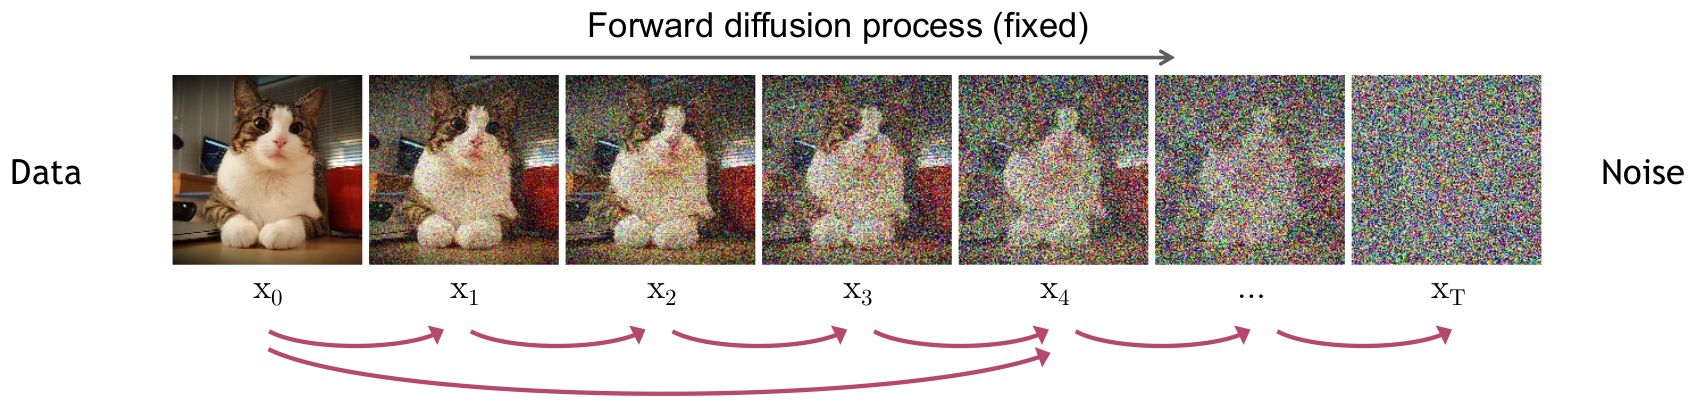
\includegraphics[width=0.9\textwidth]{assets/images/passaggio_anno/forward_diffusion_process.png}
    \end{figure}
    
\end{enumerate}


\end{frame}
%-----------------------------------



%-----------------------------------
\begin{frame}

\frametitle{Background: Score Based Diffusion Models}


\begin{enumerate}

\setcounter{enumi}{1}
    \item Learn the noise-dependent score: $\myvec{s}(\myvec{x}_t,t) := \nabla_{\myvec{x}_t} \ln{p(\myvec{x}_t)}$.

    The most popular method for estimating the score is \textbf{denoising score matching}: it uses corrupted data samples in order to estimate the score of the distribution for different levels of added noise, using a denoising neural network. %which is in practice necessary for sampling in high dimensional spaces \cite{song2019generative}. 
    $$\mathbb{E}_{t\sim u(0,1), \myvec{x}_0 \sim p(\myvec{x}_0), \myvec{x}_t \sim p(\myvec{x}_t|\myvec{x}_0)} \norm{\myvec{s}_\theta(\myvec{x}_t,t) - \nabla_{\myvec{x}_t} \ln{p(\myvec{x}_t | \myvec{x}_0)}}$$

    After training: $\myvec{s}_\theta(\myvec{x}_t,t) \approx \nabla_{\myvec{x}_t} \ln{p(\myvec{x}_t)}$
        
    
    \begin{figure}[htbp!]
    \centering    
    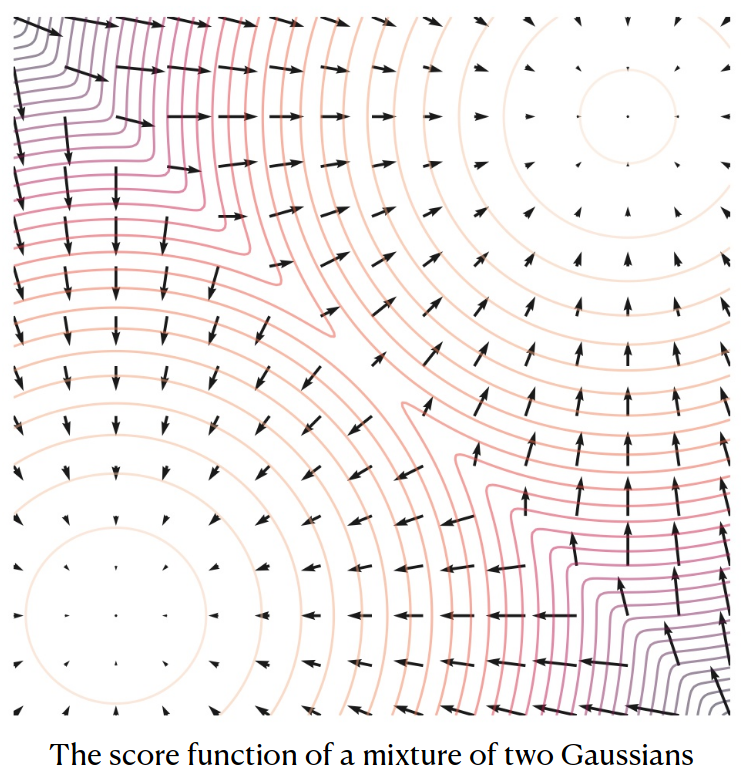
\includegraphics[width=0.3\textwidth]{assets/images/passaggio_anno/score.png}
    \end{figure}
    
\end{enumerate}

\end{frame}
%-----------------------------------



%-----------------------------------
\begin{frame}

\frametitle{Background: Score Based Diffusion Models}

\begin{enumerate}

\setcounter{enumi}{2}
    \item Use any sampling technique that uses the score to reverse the diffusion process, as annealed Langevin dynamics (\cite{song2019generative}), denoising diffusion probabilistic models (\cite{ho2020denoising}) or stochastic differential equations (\cite{sde}).

    \begin{figure}[htbp!] 
    \centering    
    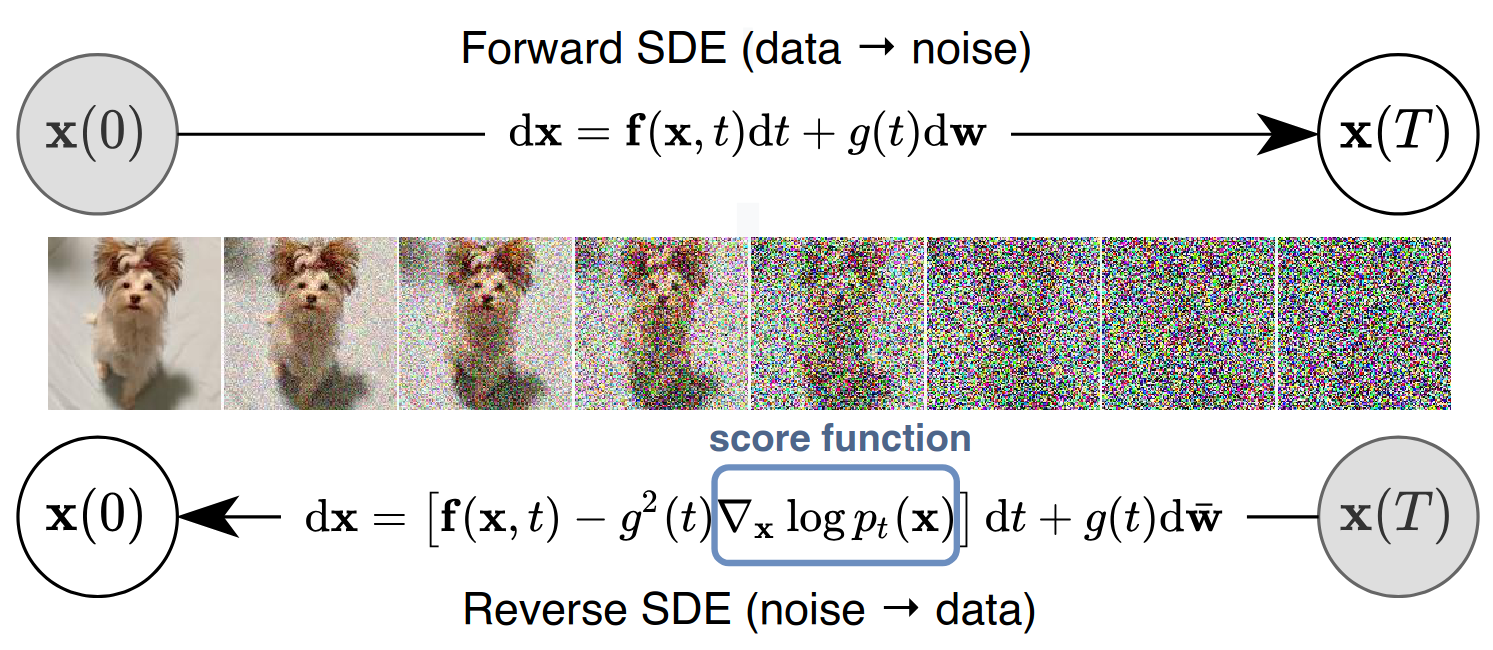
\includegraphics[width=0.75\textwidth]{assets/images/passaggio_anno/sde.png}
    \end{figure}
    
\end{enumerate}

\end{frame}
%-----------------------------------


%-----------------------------------
% these models aim at estimating the score: $\myvec{s}(\myvec{x}) := \nabla_\myvec{x} \ln{p(\myvec{x})}$

% then use sampling techniques that exploit the knowledge of the score of the distribution.

% There are several methods for estimating the score: score matching \cite{hyvarinen2005estimation}, sliced score matching \cite{song2020sliced}, and denoising score matching \cite{vincent2011connection}. Denoising score matching is probably the most popular one, it uses corrupted data samples $\tilde{\myvec{x}}$ in order to estimate the score of the distribution for different levels of added noise, which is in practice necessary for sampling in high dimensional spaces \cite{song2019generative}.

% Given a neural network $\myvec{s}_\theta(\myvec{x},t)$ and a diffusion process $q_t(\tilde{\myvec{x}} | \myvec{x})$ defined for $t \in [0,1]$ such that $q_0(\tilde{\myvec{x}} | \myvec{x}) \approx \deltx$ (no corruption) and $q_1(\tilde{\myvec{x}} | \myvec{x})$ is a fixed prior distribution (e.g., a Gaussian), the denoising score matching loss is:
% $$\mathbb{E}_{t\sim u(0,1), \myvec{x} \sim p(\myvec{x}), \tilde{\myvec{x}} \sim q_t(\tilde{\myvec{x}}|\myvec{x})} \norm{\myvec{s}_\theta(\tilde{\myvec{x}},t) - \nabla_{\tilde{\myvec{x}}} \ln{q_t(\tilde{\myvec{x}} | \myvec{x})}}$$
% %where $t\sim u(0,1)$, $x_0 \sim p(x)$, $x_t \sim q(x_t|x_0)$ and 

% With sufficient data and model capacity, denoising score matching ensures $\myvec{s}_\theta(\myvec{x},t) \approx \nabla_{\myvec{x}} \ln{p_t(\myvec{x})}$ for almost all $\myvec{x}$ and $t$, where $p_t(\myvec{x}) := \int{q_t(\myvec{x} | \myvec{x}_0)p_0(\myvec{x}_0)d\myvec{x}_0}$ is the distribution of the data for different levels of added noise.
% Given the estimate of the time/noise dependent score $\myvec{s}_\theta(\myvec{x},t)$, one can resort to different techniques for sampling from $p(\myvec{x}) = p_0(\myvec{x})$ as annealed Langevin dynamics \cite{song2019generative}, denoising diffusion probabilistic models \cite{ho2020denoising} or stochastic differential equations \cite{sde}, a generalization of the aforementioned approaches.

%-----------------------------------


%-----------------------------------
\begin{frame}

\frametitle{Background: Conditional Generation}

Given a joint distribution $p(\myvec{x}, \myvec{y})$, one is often interested in sampling from the conditional distribution $p(\myvec{x} | \myvec{y})$, where $\myvec{y}$ is for example a label. \pause

\begin{itemize}[<+->]

    \item Main approach: train a conditional score $\nabla_{\myvec{x}_t} \ln{p(\myvec{x}_t | \myvec{y})}$

    \item Alternatively, do guidance with a noise-dependent classifier $p(\myvec{y} | \myvec{x}_t)$ (\cite{dhariwal2021diffusion}):
    $$\nabla_{\myvec{x}_t} \ln{p(\myvec{x}_t | \myvec{y})} = \nabla_{\myvec{x}_t} \ln{p(\myvec{x}_t)} + \nabla_{\myvec{x}_t} \ln{p(\myvec{y} | \myvec{x}_t)}$$

    \item But if we want a model that can be conditioned by any logical constraint,  conditional training for every possible logical formula is unfeasible.
    
\end{itemize}

\end{frame}
%-----------------------------------


\begin{frame} %-----------------------------------

\frametitle{Problem formalization}

\begin{itemize}[<+->]
    \item Problem: Given the unconditional score $\nabla_{\myvec{x}_t} \ln p(\myvec{x}_t)$ and a logical constraint $\pi(\myvec{x}): \mathbb{R}^d \rightarrow \{0,1\}$, sample from 

$$ p(\myvec{x} | \pi) \propto p(\myvec{x})\pi(\myvec{x})$$



    \item \textbf{Continuous relaxation}: Given a differentiable constraint $c(\myvec{x}): \mathbb{R}^d \rightarrow (-\infty, 0]$ expressing the degree of satisfaction, sample from
    $$p_c(\myvec{x}) \propto p(\myvec{x})e^{c(\myvec{x})}$$

    
\end{itemize}

\end{frame} %-----------------------------------


% \begin{frame} %-----------------------------------

% \frametitle{Problem formalization}

% Sample from 

% $$ p(\myvec{x} | \pi) \propto p(\myvec{x})\pi(\myvec{x})$$

% Given the unconditional score $\nabla_{\myvec{x}_t} \ln p(\myvec{x}_t)$ and a logical constraint $\pi(\myvec{x}): \mathbb{R}^d \rightarrow \{0,1\}$

% \begin{itemize}
%     \item a score based generative model that samples from $p(\myvec{x})$
%     \item a logical constraint $\pi(\myvec{x}): \mathbb{R}^d \rightarrow \{0,1\}$, such that $\pi(\myvec{x})=1$ when the property is satisfied and $\pi(\myvec{x})=0$ otherwise.
% \end{itemize}

% The objective is to generate samples from $p(\myvec{x})$ that satisfy $\pi(\myvec{x})$, more formally we want to sample from the product:

% $$ p(\myvec{x} | \pi) \propto p(\myvec{x})\pi(\myvec{x})$$

% \end{frame} %-----------------------------------


% \begin{frame} %-----------------------------------
% \frametitle{Continuous relaxation}

% Instead of hard constraints $\pi(\myvec{x}): \mathbb{R}^d \rightarrow \{0,1\}$ we consider differentiable constraints (soft constraints)
% $$c(\myvec{x}): \mathbb{R}^d \rightarrow (-\infty, 0]$$
% so that the target distribution is:
% $$p_c(\myvec{x}) \propto p(\myvec{x})e^{c(\myvec{x})}$$

% \end{frame} %-----------------------------------


% \begin{frame} %-----------------------------------
% \frametitle{Method}

% The objective is to sample from $p_c(\myvec{x}) \propto p(\myvec{x})e^{c(\myvec{x})}$, given the unconditional score $\nabla_{\myvec{x}_t} \ln{p(\myvec{x}_t)}$ and constraint $c(\myvec{x})$.

% In order to do this we need the conditional noise-dependent score $$\nabla_{\myvec{x}_t} \ln{p_c(\myvec{x}_t)}$$
% %where 
% %$$p_c(\myvec{x}_t) := \int{q(\myvec{x}_t|\myvec{x}_0) p_c(\myvec{x}_0) d\myvec{x}_0}$$

% \end{frame} %-----------------------------------


\begin{frame} %-----------------------------------
\frametitle{Method}



In order to sample from the target $p_c(\myvec{x}) \propto p(\myvec{x})e^{c(\myvec{x})}$, we need the conditional noise-dependent score $\nabla_{\myvec{x}_t} \ln{p_c(\myvec{x}_t)}$:

\pause

\begin{itemize}[<+->]
    %\item At $t=0$ (no noise) $$\nabla_{\myvec{x}_0} \ln{p_c(\myvec{x}_0)} = \nabla_{\myvec{x}} \ln{p_c(\myvec{x})} = \nabla_{\myvec{x}} \ln{\frac{p(\myvec{x})e^{c(\myvec{x})}}{Z}}$$
%$$= \nabla_{\myvec{x}} [\ln{p(\myvec{x})} + c(\myvec{x}) - \ln{Z}] = \nabla_{\myvec{x}} \ln{p(\myvec{x})} + \nabla_{\myvec{x}} c(\myvec{x})$$


    \item At $t=0$ (no noise) $$\nabla_{\myvec{x}_0} \ln{p_c(\myvec{x}_0)} = \nabla_{\myvec{x}} \ln{\frac{p(\myvec{x})e^{c(\myvec{x})}}{Z}} = \nabla_{\myvec{x}} \ln{p(\myvec{x})} + \nabla_{\myvec{x}} c(\myvec{x})$$
    
    \item At $t=1$ (only noise) one can assume $\nabla_{\myvec{x}_1} \ln{p_c(\myvec{x}_1)} = \nabla_{\myvec{x}_1} \ln{p(\myvec{x}_1)}$, since enough noise is added to make samples from $p_c(\myvec{x}_1)$ distributed as the prior.
    
    \item When $t \in (0,1)$ there is no general analytical form.
    
\end{itemize}

\end{frame} %-----------------------------------


\begin{frame} %-----------------------------------
\frametitle{Conditional score approximation}

\begin{itemize}
%     \item Given this limit, we resort to approximations $\tilde{\myvec{s}}_c(\myvec{x}_t, t)$ for $\nabla_{\myvec{x}_t} \ln{p_c(\myvec{x}_t)}$, knowing the true value of the score for $t=0$ and $t=1$:
% \begin{align}
%     \tilde{\myvec{s}}_c(\myvec{x}_0, 0) &= \myvec{s}(\myvec{x}_0, 0) + \nabla_{\myvec{x}_0} c(\myvec{x}_0) \\
%     \tilde{\myvec{s}}_c(\myvec{x}_1, 1) &= \myvec{s}(\myvec{x}_1, 1)
% \end{align}

    \item We can obtain an approximation by interpolating the two regimes:
$$\tilde{\myvec{s}}_c(\myvec{x}_t, t) = \nabla_{\myvec{x}_t} \ln p(\myvec{x}_t) + g(t) \nabla_{\myvec{x}_t} c(\myvec{x}_t)$$
where $g(t): [0,1] \rightarrow [0,1]$ satisfies $g(0) = 1$ and $g(1) = 0$.

    %\item Sampling from the target distribution then reduces to substituting the score of the base model with the modified score $\tilde{\myvec{s}}_c(\myvec{x}_t, t)$.

    \pause

    \item We mostly experimented with these two forms of $g(t)$:
\begin{itemize}
    \item \textbf{Linear}: $g(t) = 1 - t$%;

    \item \textbf{SNR}: $g(t)$ is equal to the signal-to-(signal plus noise) ratio of the diffusion kernel.
\end{itemize}

    \begin{figure}[htbp!] 
    \centering    
    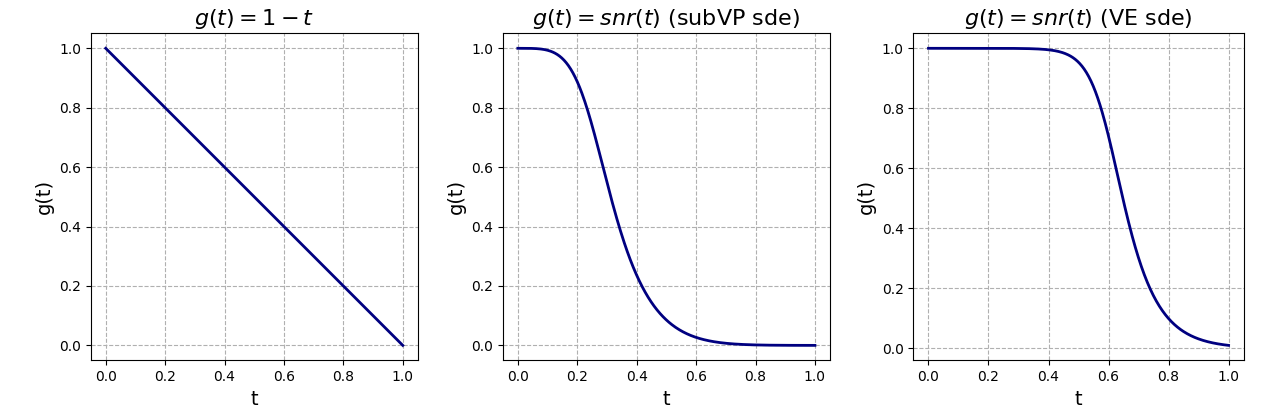
\includegraphics[width=0.8\textwidth]{assets/images/passaggio_anno/g(t).png}
    \end{figure}
\end{itemize}





\end{frame} %-----------------------------------

\begin{frame} %-----------------------------------
\frametitle{Conditional Score Approximation}

\begin{itemize}

    \item We use as weighting function $g(t)$ the signal-to-(signal plus noise) ratio of the diffusion kernel.

    \begin{figure}[htbp!] 
    \centering    
    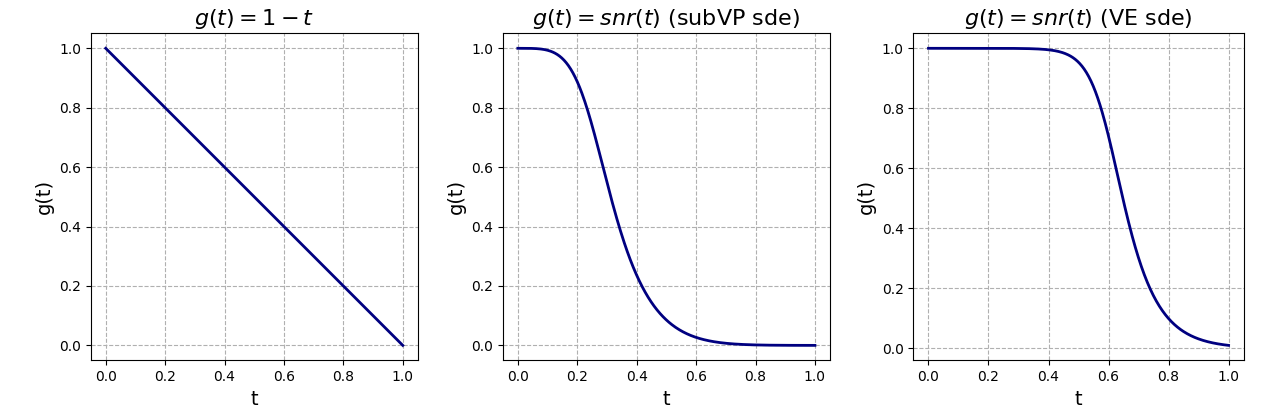
\includegraphics[width=0.7\textwidth]{assets/images/passaggio_anno/g(t).png}
    \end{figure}

    \item Intuition: the direction given by the gradient of the constraint is more meaningful as the data gets less noisy.
    
\end{itemize}


\end{frame} %-----------------------------------


% \begin{frame} %-----------------------------------
% \frametitle{Score interpolation}

% One should choose a $g(t)$ that is strong enough to guide samples towards the modes of $p_c(\myvec{x}_0)$ but at the same time that does not disrupt the reverse diffusion process in the early steps.
% We mostly experimented with these two forms of $g(t)$:
% \begin{itemize}
%     \item \textbf{Linear}: $g(t) = 1 - t$%;

%     \item \textbf{SNR}: $g(t)$ is equal to the signal-to-(signal plus noise) ratio of the diffusion kernel.
% \end{itemize}

%     \begin{figure}[htbp!] 
%     \centering    
%     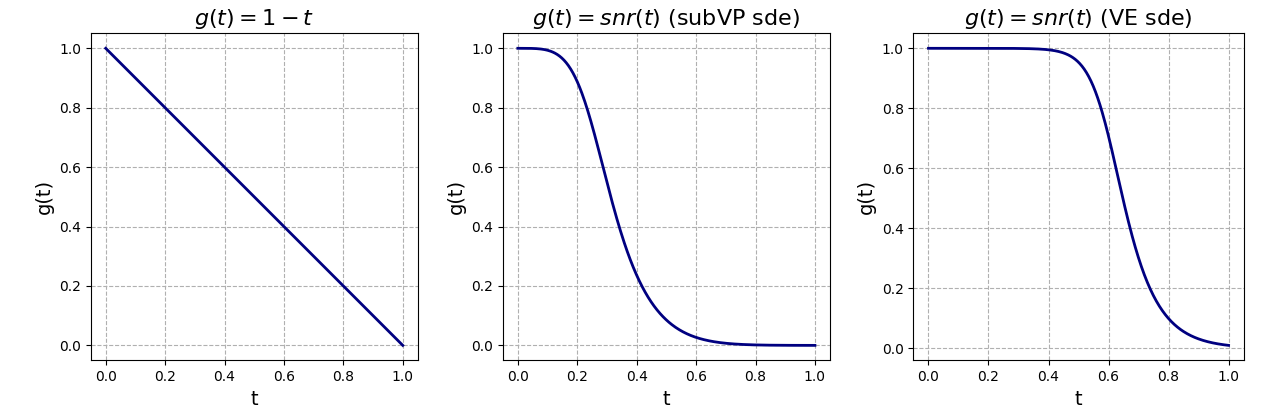
\includegraphics[width=0.8\textwidth]{assets/images/passaggio_anno/g(t).png}
%     \end{figure}

% \end{frame} %-----------------------------------


% \begin{frame} %-----------------------------------
% \frametitle{Multiple instances constraints}

% \begin{itemize}[<+->]
%     \item Sample multiple instances $(\myvec{x}_1, \ldots, \myvec{x}_n)$ that are tied together by a single multivariate constraint $c(\myvec{\myvec{x}_1, \ldots, \myvec{x}_n})$
    
%     \item $p_c(\myvec{x}_1, \ldots, \myvec{x}_n) \propto 
% p(\myvec{x}_1, \ldots, \myvec{x}_n) e^{c(\myvec{x}_1, \ldots, \myvec{x}_n)}
% = e^{c(\myvec{x}_1, \ldots, \myvec{x}_n)} \prod_{i=1}^n p(\myvec{x}_i)$

%     \item Ex: \textit{"Sample two MNIST images whose digit labels sum up to 10"}

%     \item The approximated score for each instance $\myvec{x}_i$, $i \in \{1, \ldots, n\}$ is:
% $$\tilde{\myvec{s}}_c(\myvec{x}_i, t) = \myvec{s}(\myvec{x}_i, t) + g(t) \nabla_{\myvec{x}_i} c(\myvec{x}_1, \ldots, \myvec{x}_n)$$
% \end{itemize}

% \end{frame} %-----------------------------------


% \begin{frame} %-----------------------------------
% \frametitle{Langevin dynamics correction}

% We found it useful to perform additional Langevin dynamics steps at time $t = 0$ when the score of the constrained target distribution is known without approximation.

% Langevin dynamics can be used as a Monte Carlo method for sampling from a distribution when only the score is known:

% $$ \myvec{x}^{i+1} = \myvec{x}^i + \epsilon \,\tilde{\myvec{s}}_c(\myvec{x}, 0) + \myvec{z}^i \sqrt{2 \epsilon}$$
% $$\text{where} \ \myvec{z}^i \sim \mathcal{N}(0,\mathbf{I})$$

%     \begin{figure}[htbp!] 
%     \centering    
%     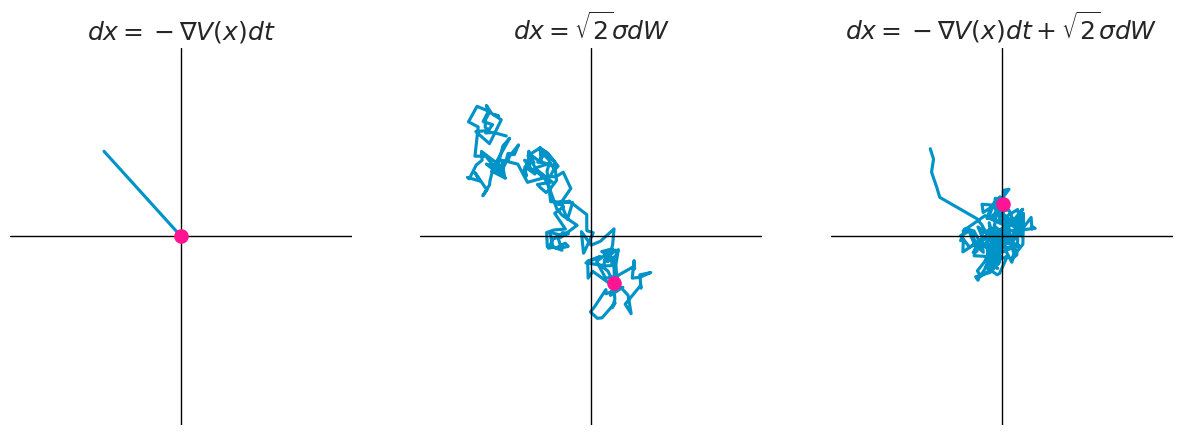
\includegraphics[width=0.7\textwidth]{assets/images/passaggio_anno/langevin_dynamics.png}
%     \end{figure}


% \end{frame} %-----------------------------------

\begin{frame} %-----------------------------------
\frametitle{Relaxing Logical Constraints}

\begin{itemize}[<+->]
    \item The score approximation needs a differentiable constraint, but logical constraints are hard and not differentiable.
    
    \item Then, we need to relax logical constraint into soft, differentiable constraints.

    \item We do this following a Neuro-Symbolic approach.
\end{itemize}

\end{frame} %-----------------------------------


\begin{frame} %-----------------------------------
\frametitle{Neuro-symbolic logical constraints}

\begin{itemize}
    \item Every atomic predicate and logical connector is associated to a differentiable function (similar to \cite{Badreddine2023logLTNDF}):

    \begin{figure}
        \centering
        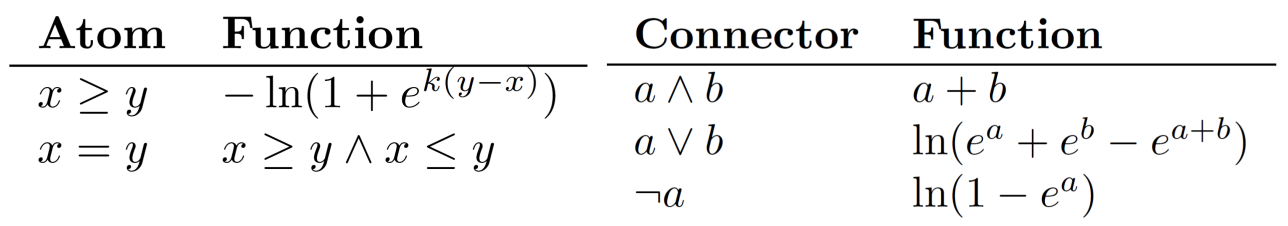
\includegraphics[width=0.8\textwidth]{assets/images/passaggio_anno/log_prob_logic.png}
    \end{figure}


    \item Connectors are based on probabilistic operations in log-space.

    \item For numerical stability it is necessary to reduce formulas to the negative normal form (NNF).

    \item This set of functions has desirable properties: exact
NNF (De Morgan's laws), numerical stability, tunable hardness ($k$).
\end{itemize}

\end{frame} %-----------------------------------


% \begin{frame} %-----------------------------------
% \frametitle{Other details}

% \begin{itemize}

% \item Constraints can involve multiple instances $c(\myvec{x}_1, \ldots, \myvec{x}_n)$:
% $$\tilde{\myvec{s}}_c(\myvec{x}_i, t) = \myvec{s}(\myvec{x}_i, t) + g(t) \nabla_{\myvec{x}_i} c(\myvec{x}_1, \ldots, \myvec{x}_n)$$

% \item Langevin dynamics at $t=0$ (exact score):

%     \begin{figure}[htbp!] 
%     \centering    
%     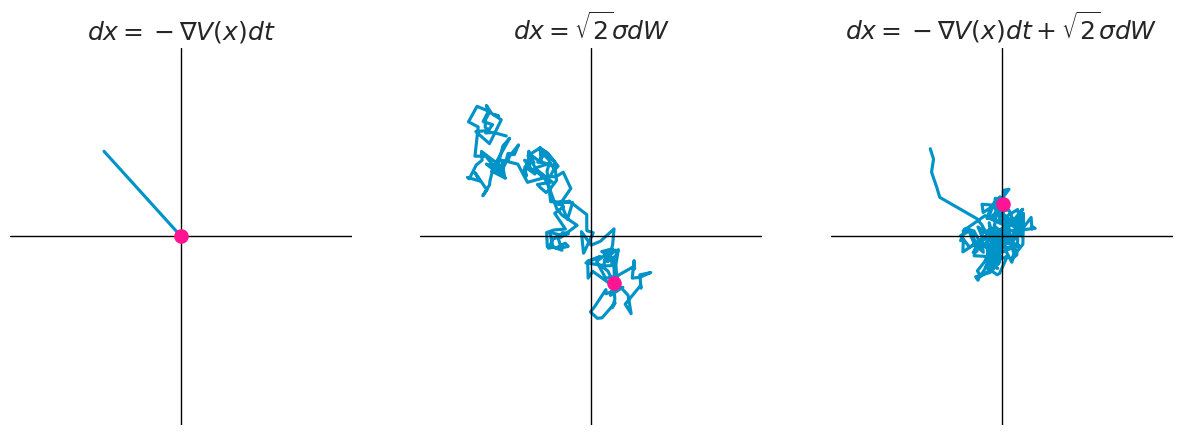
\includegraphics[width=0.7\textwidth]{assets/images/passaggio_anno/langevin_dynamics.png}
%     \end{figure}


% \item Estimation of score at $t=0$ with denoising score matching is problematic, so we employed some tricks to improve it.
% \end{itemize}

% \end{frame} %-----------------------------------


% \begin{frame} %-----------------------------------
% \frametitle{Training a score model for tabular data}

% \begin{itemize}
%     \item Correctly estimating the score at $t=0$ is difficult
%     \item We improved the score estimate mainly by parametrizing carefully the score network and using large batches.
%     \item Correctly estimating the score at $t\approx0$ is fundamental to make our method work in practice, since it allows us to perform Langevin MCMC at $t\approx0$, where the conditional score is known without approximation.
% \end{itemize}

% \end{frame} %-----------------------------------

%-----------------------------------
\begin{frame}

\frametitle{Zero-Shot Conditional Sampling}

\textbf{Input}: pre-trained score-based diffusion model for $p(\myvec{x})$ and a user defined logical constraint $\pi$.
\newline
\textbf{Output}: conditional samples from $p(\myvec{x} | \pi)$

\begin{enumerate}

    \item Convert the logical constraint to a soft, differentiable constraint using the neuro-symbolic framework
    
    \item Approximate the conditional score by applying the approximation to the original score and the neuro-symbolic constraint 

    \item Plug the approximated conditional score in the original score-based sampling algorithm to generate new points

\end{enumerate}

Notice that this method doesn't require any training!


\end{frame}
%-----------------------------------

\begin{frame} %-----------------------------------
\frametitle{Experiments}

\begin{itemize}
    \item Data: tabular, time series, images
    \item Baseline: rejection sampling (RS) when possible
    \item Metrics for comparing two samples $X$ and $Y$:
    \begin{itemize}
        \item Average l1 distance in correlation coefficients.
        \item Total variation distance: $ D(X,Y):=\frac{1}{2} \sum_i |x_i - y_i|$ where $x_i$ and $y_i$ are the empirical probabilities for a given common binning. This distance is upper bounded by 1. Intuitively, it's the area of each of the two histograms that is not shared.
    \end{itemize}
    %\item Pre-trained unconditional models were used when possible, otherwise they were trained using SDEs. 
    %\item Comparison with \cite{bansal2023universal}
\end{itemize}

\end{frame} %-----------------------------------


\begin{frame} %-----------------------------------
\frametitle{Experiments: tabular data}

Datasets:
\begin{itemize}
    \item White wine dataset (\cite{misc_wine_quality_186}): 11 numerical dimensions ($\mathbb{R}^{11}$).
    \item Adult (\cite{misc_adult_2}): 5 numerical and 10 categorical dimensions.
\end{itemize}

Unconditional score-based model are trained using SDEs (\cite{sde}). Categorical variables were embedded in continuous space using one-hot encodings.

\end{frame} %-----------------------------------


\begin{frame} %-----------------------------------
\frametitle{Experiments: tabular data}

\begin{enumerate}
    \item White wine, \texttt{$(\text{fixed acidity} \in [5.0, 6.0]  \lor  \text{fixed acidity} \in [8.0, 9.0]) \land \text{alcohol} \geq 11.0 \land (\text{residual sugar} \leq 5.0 \rightarrow \text{citric acid} \geq 0.5)$}

    \begin{figure}[htbp!] 
    \centering    
    
\includegraphics[width=0.6\textwidth]{.materiale/articles/zero_shot_conditional_generation/images/white_wine_compressed.pdf}
    \end{figure}
    
\end{enumerate}


\end{frame} %-----------------------------------


\begin{frame} %-----------------------------------
\frametitle{Experiments: tabular data}

\begin{enumerate}
\setcounter{enumi}{1}
    \item White wine, \texttt{$\text{alcohol}_1 > \text{alcohol}_2 + 1$}
    \item Adult, \texttt{$\text{age} \geq 40 \land (\text{race} \neq \text{"White"} \lor \text{education} = \text{"Masters"})$}
\end{enumerate}

\begin{table}[ht]
\centering
\resizebox{\textwidth}{!}{%
\begin{tabular}{@{}lcccccc@{}}
\toprule
\textbf{Experiment} &
  \textbf{Avg TV} &
  \textbf{Max TV} &
  \textbf{Avg L1 corr} &
  \textbf{Hard sat} &
  \multicolumn{1}{c}{\textbf{Hard sat (RS)}} &
  \multicolumn{1}{c}{\textbf{RS acc. rate}} \\ \midrule
White wine        & 0.1   & 0.153 & 0.07  & 86\%  & 92\%  & 1.67\% \\
White wine (multi) & 0.061 & 0.086 & 0.027 & 99\%  & 100\% & 27\%   \\
Adult             & 0.067 & 0.13  & 0.046 & 100\% & 100\% & 1.73\% \\ \bottomrule
\end{tabular}%
}
\end{table}

\begin{itemize}
    \item In general low error for simple constraints, still acceptable for complex constraints.
    \item This methods allow to sample more efficiently in low probability regions.
\end{itemize}

\end{frame} %-----------------------------------




% \begin{frame} %-----------------------------------
% \frametitle{Experiments: time series}

% \begin{itemize}
%     \item Dataset: Simulated eSIRS time series (spreading of a disease in an open population). Fixed population of size $N$ composed of Susceptible ($S$), Infected ($I$), and Recovered ($R$) individuals.

%     \begin{figure}
%         \centering
%         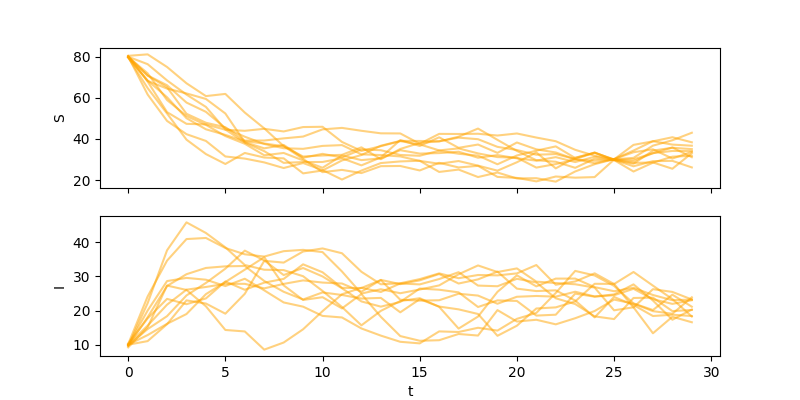
\includegraphics[width=0.65\linewidth]{assets/images/passaggio_anno/eSIRS.png}
%     \end{figure}

%      \pause

%     \item Consistency constraints:

%     \begin{itemize}
%     \item \textit{Non-negative populations}: $\forall t \ S(t) \geq 0 \land I(t) \geq 0$
%     \item \textit{Constant population}: $\forall t \ S(t)+I(t) \leq N$
% \end{itemize}

%      \pause

%     \item Additional constraints...
% \end{itemize}

% \end{frame} %-----------------------------------




\begin{frame} %-----------------------------------
\frametitle{Experiments: time series}
    
    Dataset: Simulated eSIRS time series (spreading of a disease in an open population). Fixed population of size $N$ composed of Susceptible ($S$), Infected ($I$), and Recovered ($R$) individuals.

    \vspace{2mm}
    
\begin{columns}

    \begin{column}{0.5\textwidth}
        \centering
        \small{$\forall t \ I(t) \leq 20$}
        
\includegraphics[width=0.9\textwidth]{.materiale/articles/zero_shot_conditional_generation/images/eSIRS_inequality.pdf}
    \end{column}

    \begin{column}{0.5\textwidth}
        \centering
        \small{$S(0)=95 \land I(0)=5 \land S(25)=30$}
        
\includegraphics[width=0.9\textwidth]{.materiale/articles/zero_shot_conditional_generation/images/eSIRS_bridging.pdf}
    \end{column}
    
\end{columns}

\begin{itemize}
    \item High satisfaction rate, low error (When RS was possible)
\end{itemize}

\end{frame} %-----------------------------------






\begin{frame} %-----------------------------------
\frametitle{Experiments: images}

\begin{itemize}[<+->]

    \item Image symmetry:

    \begin{figure}[htbp!] 
    \centering    
    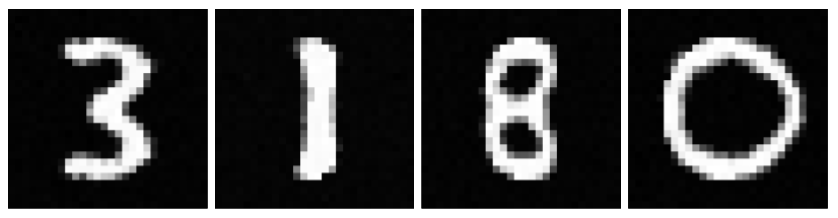
\includegraphics[width=0.5\textwidth]{assets/images/passaggio_anno/mnist_symmetry.png}
    \end{figure}

    \begin{figure}[htbp!] 
    \centering    
    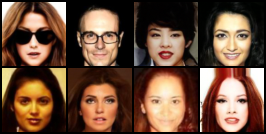
\includegraphics[width=0.5\textwidth]{assets/images/passaggio_anno/celebA_symmetry.png}
    \end{figure}

    Not really effective, one have to trade-off sample quality and constraint satisfaction by tuning the constraint strenght $k$.

\end{itemize}
\end{frame} %-----------------------------------



\begin{frame} %-----------------------------------
\frametitle{Experiments: images}

\begin{itemize}[<+->]


    \item Image restoration (with known corruption process $f$):

    $$\forall i \ f(\myvec{x})_i = \tilde{\myvec{y}}_i$$

    \begin{figure}[htbp!] 
    \centering    
    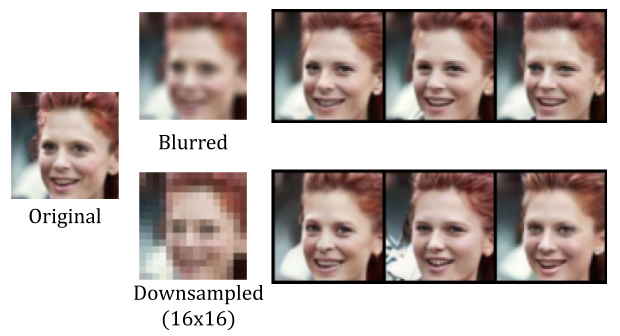
\includegraphics[width=0.7\textwidth]{assets/images/passaggio_anno/celebA_restoration.png}
    \end{figure}

    
\end{itemize}
\end{frame} %-----------------------------------



\begin{frame} %-----------------------------------
\frametitle{Experiments: images}

\begin{itemize}[<+->]

    \item MNIST digits sum: \textit{"Sample two MNIST images whose digit labels sum up to 10"}

    $$\bigvee_{i=1}^{9} \text{{class}}(\myvec{x}, i) \land \text{{class}}(\myvec{y}, 10-i) $$

        Where "class" is a pretrained classifier.


    \begin{figure}[htbp!] 
    \centering    
    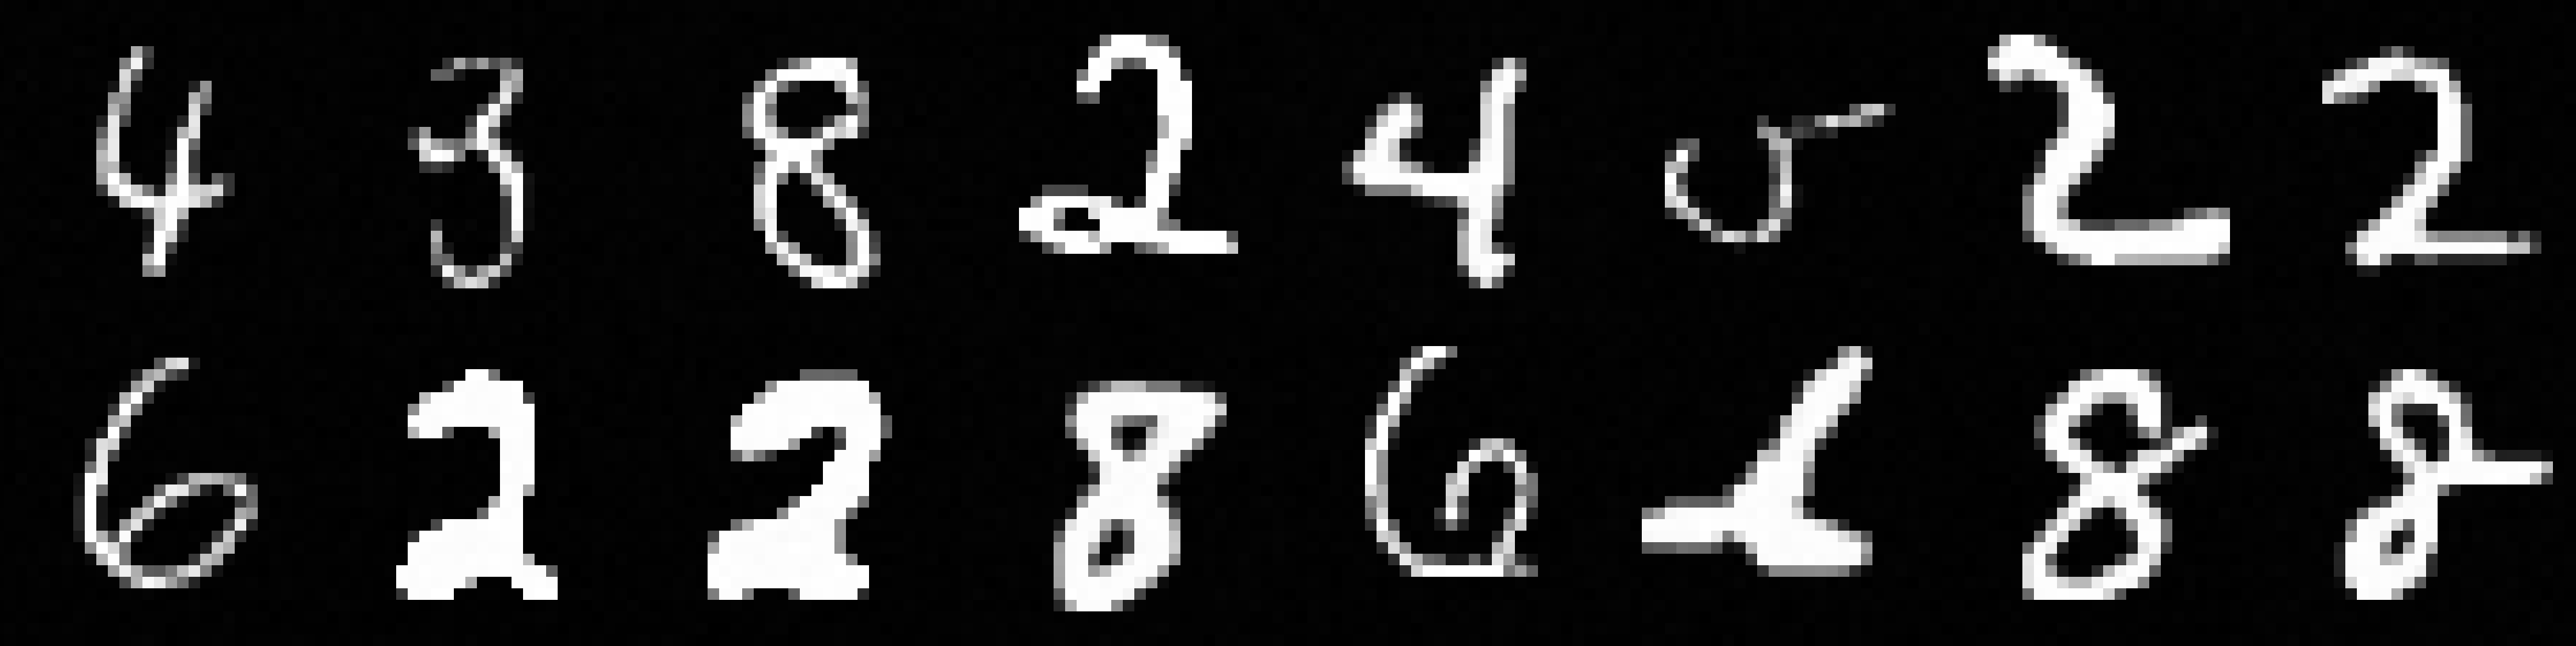
\includegraphics[width=0.8\textwidth]{assets/images/passaggio_anno/mnist_digits_sum.png}
    \end{figure}


    According to the classifier $\approx 96\%$ of pairs sum up to 10, but only 2-8, 6-4 pairs are generated.
\end{itemize}
\end{frame} %-----------------------------------



\begin{frame} %-----------------------------------
\frametitle{Comparison with Universal Guidance}

\begin{itemize}
    \item Universal Guidance (\cite{bansal2023universal}) is probably the state of the art for plug-and-play conditioning.

    \item Originally applied to imaging problems.

    \item Oversimplifying, it involves at each time step an optimization of the denoising prediction $\myvec{x}_0$ (that is a linear transformation of the score), in order to make it satisfy the constraint $c(\myvec{x}_0)$.

    
    \item It fails in two of the tasks we tested:

    \begin{table}[ht]
    
\begin{tabular}{@{}lcccc@{}}
\toprule
\multicolumn{1}{c}{\multirow{2}{*}{Method}} & \multicolumn{2}{c}{White wine} & \multicolumn{2}{c}{eSIRS bridging} \\ \cmidrule(l){2-5} 
\multicolumn{1}{c}{} & \textbf{Avg TV} & \textbf{Max TV} & \textbf{Avg TV} & \textbf{Max TV} \\ \midrule
\textbf{Ours}        & \textbf{0.1}    & \textbf{0.15}  & \textbf{0.13}  & \textbf{0.25}  \\
Univ. Guidance                   & 0.29           & 0.85           & 0.47           & 1.0             \\ \bottomrule
\end{tabular}
%\caption{Comparison with Universal Guidance. On the first white wine and eSIRS bridging tasks our method performs significantly better in terms of Total variation distance (we report average and maximum distance over the marginals).}\label{tab:universal_guidance_comparison_short}
\end{table}

\end{itemize}

\end{frame} %-----------------------------------


\begin{frame} %-----------------------------------
\frametitle{Experiments: comparison with Universal Guidance}

\begin{itemize}

    \item It performs better on image problems:
    $$\bigvee_{i=1}^{9} \text{{class}}(\myvec{x}, i) \land \text{{class}}(\myvec{y}, 10-i) $$

    \begin{figure}[htbp!] 
    \centering    
    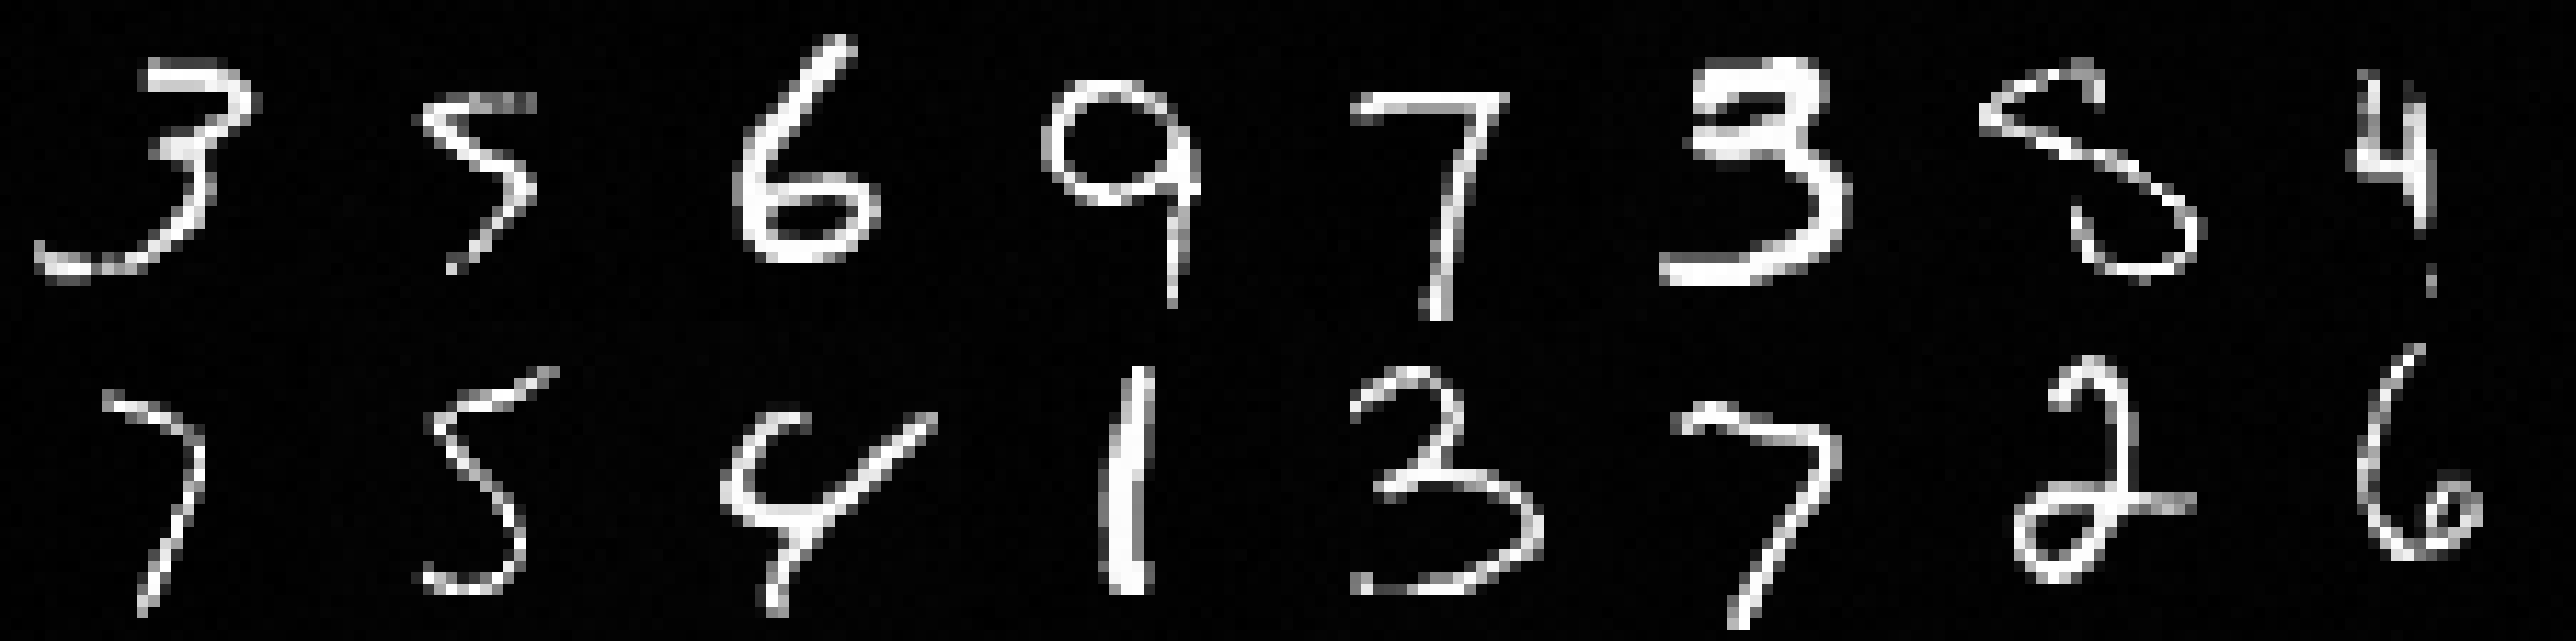
\includegraphics[width=0.8\textwidth]{assets/images/passaggio_anno/mnist_digits_sum_universal_guidance.png}
    \end{figure}

    \item It is able to generate high quality samples but it misses the correct approximation of the conditional distribution, probably because it involves an optimization phase.  

\end{itemize}

\end{frame} %-----------------------------------



\begin{frame} %-----------------------------------
\frametitle{Discussion}

\begin{itemize}[<+->]

    \item Our method is SOTA for zero-shot conditional distribution approximation on tabular data with logical constraints.

    \item Nevertheless, as complexity increases, it is necessary to trade-off constraint satisfaction with samples quality.

    \item When it is more important to obtain high quality samples, rather than approximating the true conditional distribution, other methods are to be preferred.
    
    \item Conditional score approximation can be improved, by taking inspiration from recent zero-shot methods for images, but fixing the problem with optimization.
    
\end{itemize}

\end{frame} %-----------------------------------
